\documentclass{mpaper}

\begin{document}

\title{Measuring Software Ticket Quality using Statistical Analysis}
\author{Andrei-Mihai Nicolae}
\matricnum{2147392}

\maketitle

\begin{abstract}
Software tickets are of valuable importance to the whole computing science 
field - they guide engineers towards better planning, management 
and tracking of their progress throughout complex projects. However, there
are few studies that investigate what makes for a high quality,
valuable ticket. This can lead to multiple issues in a company, such as 
increased communication friction between developers and end users filing bug
reports, as well as increased overall costs due to waste of development effort. 
In this research paper, we present our findings after 
investigating a large number of variables surrounding software tickets, 
such as whether the presence of stack traces influence the time 
to close for the ticket. Our results show that the presence and type of attachments,
comments complexity (i.e. number of comments per ticket), grammar correctness scores
as well as the sentiment drawn from the comments can influence the quality of the ticket.
We bring a couple of novel aspects to the research
community including one of the largest dataset statistically analysed in the field,
as well as state-of-the-art sentiment and grammar correctness analysis.
\end{abstract}

\section{Introduction}

In the past decade, technology has drastically increased its influence on 
virtually every aspect of our society. Therefore, software projects have 
inherently become more complex and require increasing number of developers in
the team. Due to this, software engineers have created issue tracking systems,
a means of planning, managing and tracking work products in the form of 
\emph{software tickets} or \emph{issues}.

There are multiple platforms for providing such issue tracking systems, among which
the most popular are Jira \cite{jira} and Bugzilla \cite{bugzilla}. For both platforms,
the tickets are split into two main categories: feature requests (i.e. feature to be 
implemented into the system) and bug reports (i.e. issue encountered by an end user or
discovered by a developer in the codebase). Regardless of the type of ticket, they provide
various types of information that can be filled in by the reporter, including:
  \begin{itemize}
    \item summary - short description of the feature to be implemented/encountered bug;
    \item description - longer textual field which goes into more detail regarding the ticket;
    it can include various types of information, such as stack traces or steps to reproduce a bug;
    \item attachments - screenshots, snippets of code or configuration files that might help
    close the ticket faster;
    \item comments - each ticket can have any number of comments where the people interested in 
    it can talk about what might have caused the bug, how to fix it etc.
  \end{itemize}

Even though tickets provide such comprehensive information regarding a specific task, studies have shown 
that fixing bugs is one of the most common tasks performed by developers \cite{latoza2006maintaining}. One of
the reasons for this is the communication friction between developers and end users \cite{Korkala2014WasteIdentification}
as developers might need clarification regarding what information the users have provided (e.g. cannot reproduce the bug, 
screenshot is unclear). Another main reason for this waste of effort on solving tickets, according to 
Just et. al \cite{just2008towards} and Zimmermann et. al \cite{zimmermann2009improving}, is the generally poor design of issue 
tracking systems. This can lead to various issues, including increased costs for the company, wasted development effort, 
decreased customer satisfaction and overall poor performance.

Therefore, there is a need in the community to find the answer to what makes for a high quality, valuable software ticket 
that would improve the overall performance of the development team and, inherently, the company. As there are many 
fields in a ticket, the number of unanswered questions is rather large: do stack traces have an influence on the quality
of a ticket? What about attachments and whether a screenshot is more helpful than a snippet of code? Does a negative sentiment
drawn from comments increase or decrease the time taken to solve a bug? How does grammar correctness influence the 
communication friction?

In this research paper, we present and discuss our findings after running a statistical analysis 
on over 300,000 tickets taken from more than 15 open source projects. We have implemented a Go application 
with multiple commands (i.e. store, analyze, plot, statistics) that can automatically fetch any number of tickets 
from a Jira instance, analyze them, generate plots and run statistical tests. 

During the analysis part, we investigate several variables in correlation with \emph{time-to-complete}, 
which we define as the \emph{metric of quality} (\emph{time-to-complete} represents the period of time between the creation 
and the closing of a ticket). There are multiple novel aspects brought by our study, among which is the fact that it is one of 
the very few studies that have tackled this issue using a quantitative rather than a qualitative approach (with a very 
large number of tickets analysed) and also that it uses state-of-the-art sentiment \cite{wilson2005recognizing} as well as 
grammar correctness analysis techniques \cite{wilson2005recognizing}. We believe that our results are valuable 
contributions to the research community and the database produced after the analysis can help further studies with 
analyzed and well-tested data.

\section{Related Work}

\section{Building the Data Set}

\begin{figure*}
\begin{center}
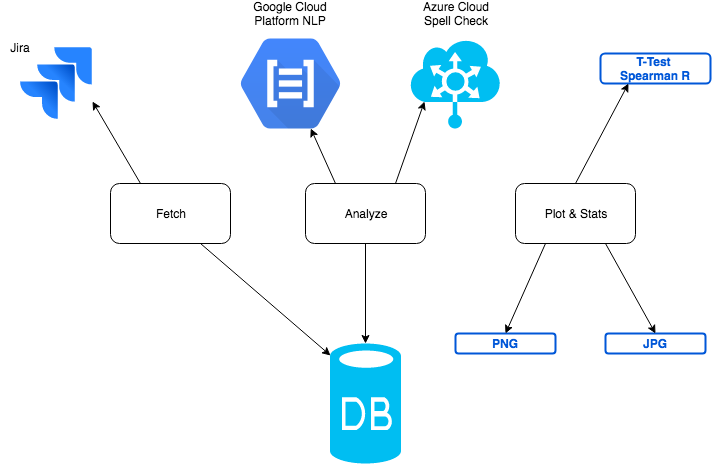
\includegraphics[scale=0.3]{images/flow.png}
\end{center}
\caption{\label{fig-eg}Flow of the whole application.}
\end{figure*}

The first step to building the data set was to create a tool that was able to execute all the commands that we required:
fetching the tickets from any Jira instance, storing them into some form of database, analyze the variables of interest, 
automatically plot the correlations between them and run statistical analysis on the data. After careful consideration, 
we decided that Go was the best way to go for various reasons:
  \begin{itemize}
    \item it is designed with simplicity in min, thus making it easier for others who might join the project to read 
    and understand the codebase;
    \item it is compiled, statically typed, which implies that it is a much faster candidate than other interpreted languages
    such as Ruby or Python;
    \item is is designed with concurrency in mind, thus it helps reduce times of execution and computing power considerably;
  \end{itemize}

Figure \ref{} The following two subsections will describe in detail how the process of building the data set was undergone.

\subsection{Fetch and Store}

This is the first command implemented in our tool - it is desgined to fetch, from any valid Jira URL, any number of tickets 
and then store everything inside an instance of BoltDB \cite{bolt}, which is a very simple yet powerful key-value pair 
database. The whole process is parallelized with the possibility of scaling even up to hundreds of goroutines
(i.e. lightweight threads) running concurrently.

In terms of projects selected, we have opted for the Apache Software Foundation which open-sourced some of the most popular
software applications. Moreover, they have all their projects' issue tracking systems hosted on Jira, thus we could also 
achieve consistency easier. 

\subsection{Analyse}

\section{Characterising the Data Set}

\subsection{Attachments}

\subsection{Comments}

\subsection{Summary and Description}

\subsection{Grammar Correctness}

\subsection{Sentiment Analysis}

\subsection{Steps to Reproduce}

\subsection{Stack Traces}

\section{Correlations}

\section{Future Work}

\section{Conclusions}

\vskip8pt \noindent
{\bf Acknowledgments.}
Tim, my parents, Corina.

\bibliographystyle{abbrv}
\bibliography{paper}


\end{document}

% \begin{table}
% \begin{tabular}{l||c||p{2cm}}
% \emph{Operating System} & \emph{Version} & \emph{Verdict} \\ \hline \hline
% Ubuntu & 12.04 & Everyone's favourite Linux, unless you grew up with
% RedHat \\ \hline
% Slackware & xxx & Pseudo-hacker's Linux, how often do you recompile
% your kernel? \\ \hline
% Mac OS & 10.7 & For people with more money than sense \\ \hline
% \end{tabular}
% \caption{\label{tab-eg}Single column table of figures}
% \end{table}

% \begin{figure*}
% \begin{center}
% 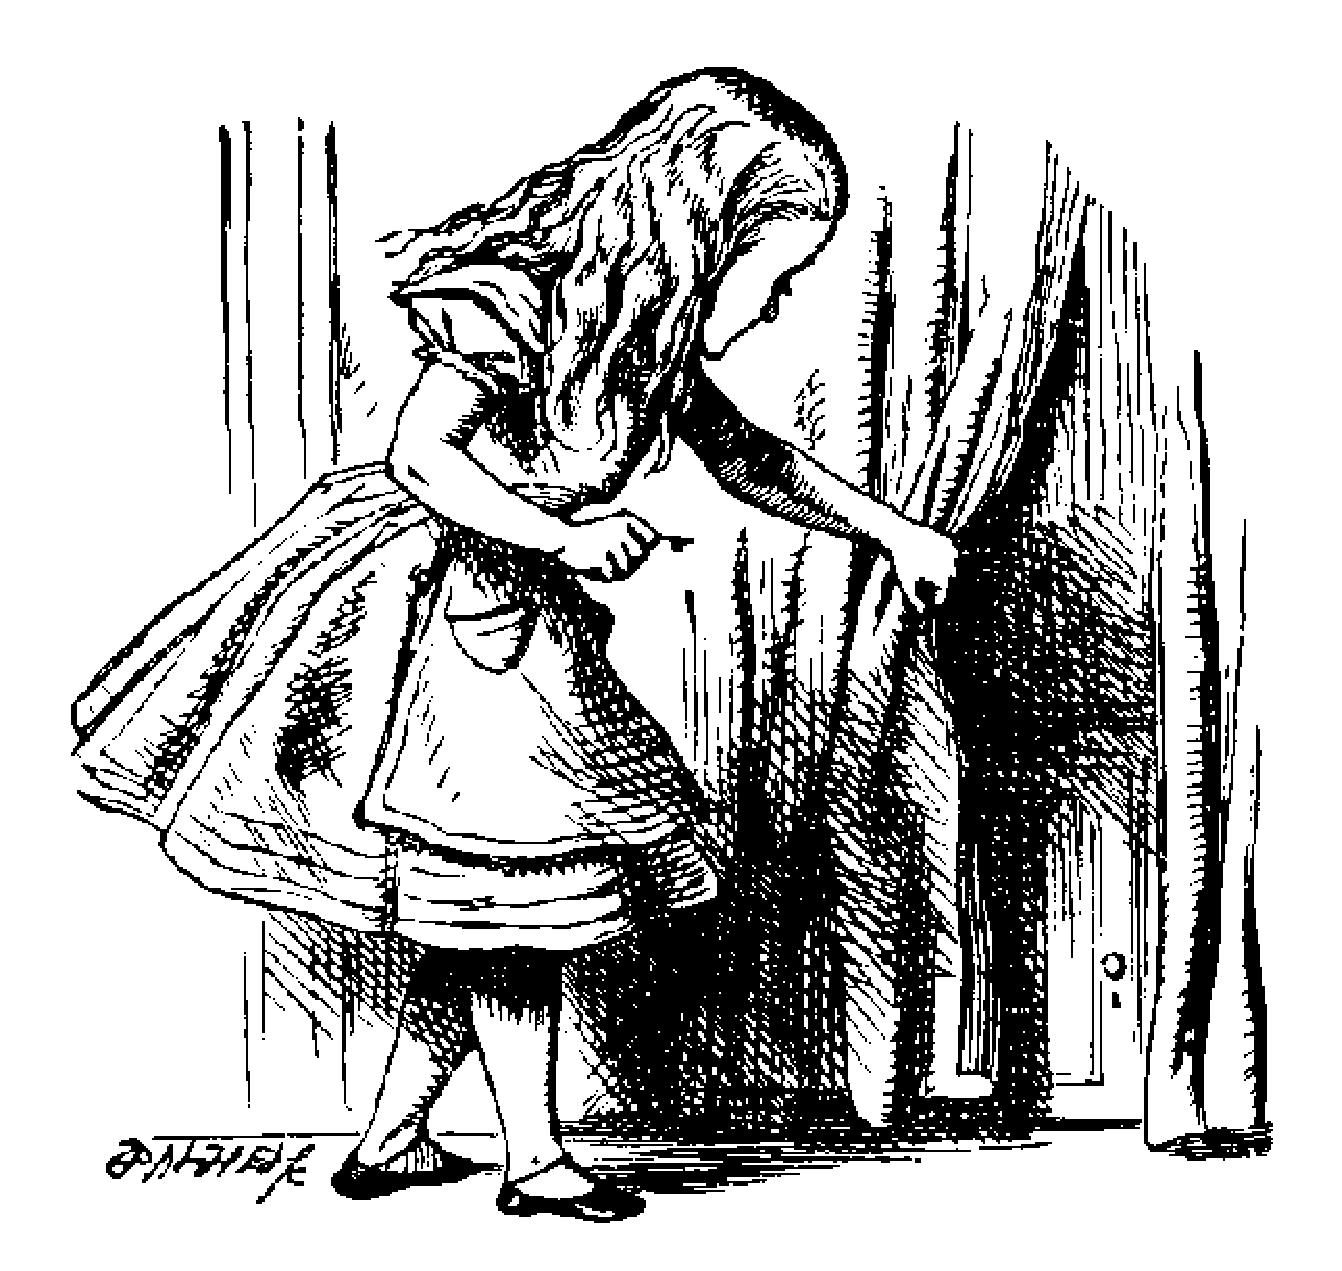
\includegraphics[scale=0.3]{images/alice.pdf}
% \end{center}
% \caption{\label{fig-eg}An example figure stretching over two columns}
% \end{figure*}